%%%%%%%%%%%%%%%%%%%%%%%%%%%%%%%%%
%
%       EXERCÍCIO
%
%%%%%%%%%%%%%%%%%%%%%%%%%%%%%%%%%

\ifdefstring{\atividade}{prova}{%
    \ifdefstring{\modo}{objetivo}{%
        \renewcommand{\valorquestao}{\ValorQObj\ ponto}
    }{%
        \renewcommand{\valorquestao}{\ValorQDisc\ pontos}
    }%
}%

\begin{exercicioBanco}[\valorquestao]
Sabendo que o gráfico a seguir representa a função \(f(x) = -|x+1| + |x-1|\), determine o valor de \(y_{1}\cdot y_{2}\).
\begin{center}
    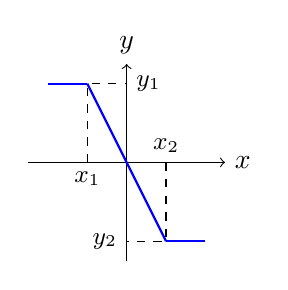
\begin{tikzpicture}[scale=0.5]
        % Eixos
        \draw[->] (-2.5,0) -- (2.5,0) node[right] {\(x\)};
        \draw[->] (0,-2.5) -- (0,2.5) node[above] {\(y\)};

        % Gráfico da função f(x) = |x-2| + |x+3|
        \draw[domain=-2:-1, thick, blue] plot (\x, {2}); % x < -1
        \draw[domain=-1:1, thick, blue] plot (\x, {-2*\x});    % x ≥ -1
        \draw[domain=1:2, thick, blue] plot (\x, {-2});    % x ≥ -1

        % Marcação do vértice (x = -1)
        \draw[dashed] (-1,0) -- (-1,2) -- (0,2);
        \node[below] at (-1,0) {\small\(x_{1}\)};
        \node[right] at (0,2) {\small\(y_{1}\)};
        \draw[dashed] (1,0) -- (1,-2) -- (0,-2);
        \node[above] at (1,0) {\small\(x_{2}\)};
        \node[left] at (0,-2) {\small\(y_{2}\)};
    \end{tikzpicture}
\end{center}


% Define as alternativas
\newcommand{\alternativas}{%
    \begin{center}
        \begin{tabularx}{\textwidth}{XXXXX}
            (a) \(-1\). &
            (b) \(-2\). &
            (c) \(-4\). &
            (d) \(-\dfrac{1}{2}\). &
            (e) \(-\dfrac{1}{4}\).
        \end{tabularx}
    \end{center}
}

% Define a resposta correta
\newcommand{\resposta}{C}

% Lógica condicional para exibição
\ifdefstring{\atividade}{lista}{%
    \alternativas
    \vspace{0.5em}
    
    \noindent\textbf{Resposta:} letra \textbf{\resposta}.
}{%
    \ifdefstring{\modo}{objetivo}{%
        \alternativas
    }{%
        % modo = discursiva → não mostra alternativas
    }
}
\end{exercicioBanco}

